\documentclass[a4paper, 12pt]{article}

\usepackage[english, russian]{babel}
\usepackage[T2A]{fontenc}
\usepackage[utf8]{inputenc}
\setlength{\parindent}{1cm}
\usepackage{graphicx}
\usepackage{amsmath}
\usepackage{amssymb}
\usepackage{amsfonts}
\usepackage{array}
\usepackage{booktabs}
\usepackage{wrapfig}
\usepackage{caption} %заголовки плавающих объектов
\captionsetup[table]{justification=centering} %установки для заголовков таблиц
\captionsetup[figure]{justification=centering} %установки для заголовков таблиц

\begin{document}

	\begin{center}
	\subsubsection*{Отчёт к лабораторной работе №27}
	
	\subsubsection*{Полосовой активный фильтр и автогенератор на операционном усилителе}
	
	\subsubsection*{Преподаватель: Петриков В. Д.}
	
	Выполнил студент третьего курса вышей школы фундаментальных физический исследований: Куликовских Илья
	
	Группа: 5030302/30801
\end{center}


\subsubsection*{Исследование пассивного RC-фильтра}

На монтажной плате нами была собрана схема исследования частотных свойств пассивного RC-фильтра (рис. 1).

\begin{figure}[htpb]
	\centering
	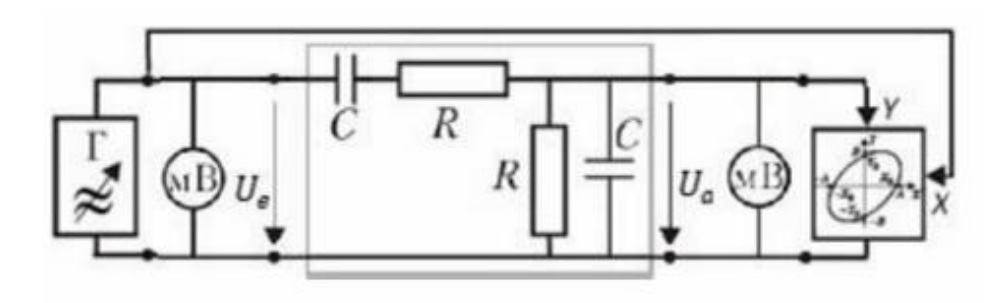
\includegraphics[width=0.8\textwidth]{27-1.png}
	\caption{Схема пассивного $RC$-фильтра}
\end{figure}

Характеристики устройств:
\[ R = 10 \, \text{кОм} \]
\[ C = 15 \, \text{нФ} \]

Центральная частота полосы пропускания (квазирезонансная частота): 
\[ f_0 = \dfrac{1}{2\pi RC} = 1061.57 \, \text{Гц} \]

Теоретический коэффициент передачи фильтра: 
\[ K = \dfrac{1}{\sqrt{3 + \left( \dfrac{f_0}{f} - \dfrac{f}{f_0} \right)^2}} \]
При \( f \rightarrow f_0 \) получаем \( K = \dfrac{1}{3} = 0.33 \)

\begin{wrapfigure}{r}{0.5\textwidth}
	\centering
	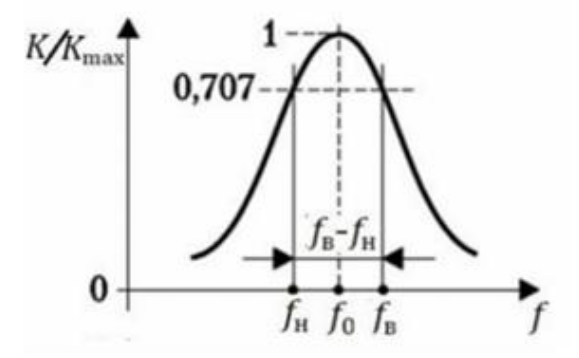
\includegraphics[width=0.5\textwidth]{27-2.png}
	\caption{AЧХ фильтра}
\end{wrapfigure}

После сборки схемы мы экспериментально определили резонансную частоту цепи. Для этого переключили осциллограф в режим XY и, регулируя частоту генератора, добились превращения фигуры Лиссажу в прямую линию.

В результате измеренная квазирезонансная частота: \( f_{0\ эксп} = 935.84 \, \text{Гц} \)

Коэффициент передачи был измерен при помощи двух вольтметров путем измерения значений входного \( U_e \) и выходного \( U_a \) напряжений и вычисления их отношения.

Входное напряжение: \( U_e = 1 \, \text{В} \)
Выходное напряжение: \( U_a = 0.3 \, \text{В} \)
Коэффициент передачи: \( K_{\text{эксп}} = \dfrac{U_a}{U_e} = 0.3 \)

Значение выходного напряжения, при котором наблюдаются верхняя и нижняя частоты среза (рис. 2): 
\[ U_p = U_a \times 0.707 = 0.21 \, \text{В} \]

Верхняя и нижняя частоты среза соответственно: 
\[ f_B = 3163.02 \, \text{Гц}; \quad f_H = 278.75 \, \text{Гц} \]

Полоса пропускания: 
\[ \Delta f = f_B - f_H = 2884.27 \, \text{Гц} \]

Добротность фильтра: 
\[ Q = \dfrac{f_{0\ эксп}}{\Delta f} = 0.32 \]

Погрешность квазирезонансной частоты: 
\[ \dfrac{f_0 - f_{0\ эксп}}{f_0} \times 100\% = 11.85\% \]
Данное значение превышает погрешность для резисторов и конденсаторов в 10\% на 1.85\%.

Погрешность коэффициента передачи: 
\[ \dfrac{K - K_{\text{эксп}}}{K} \times 100\% = 9.09\% \]
Данное значение не превышает погрешность для резисторов и конденсаторов в 10\%.

\subsubsection*{Исследование избирательного усилителя}

На монтажной плате была собрана схема RC-усилителя (рис. 3).

\begin{figure}[htpb]
	\centering
	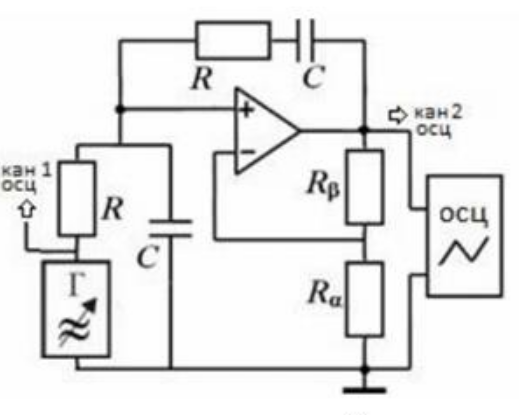
\includegraphics[width=0.5\textwidth]{27-3.png}
	\caption{Схема избирательного усилителя}
\end{figure}

Характеристики устройств:
\[ R = 10 \, \text{кОм} \]
\[ C = 15 \, \text{нФ} \]
\[ R_\alpha = 205 \, \text{Ом} \]
\[ R_\beta = 393 \, \text{Ом} \]

Коэффициент усиления HV: 
\[ k = 1 + \dfrac{R_\beta}{R_\alpha} = 2.92 \]

Дальнейшие измерения проводились по аналогии с предыдущим разделом:

Квазирезонансная частота: \( f_{0\ эксп} = 923.74 \, \text{Гц} \)

Входное напряжение: \( U_e = 0.1 \, \text{В} \)
Выходное напряжение: \( U_a = 2.55 \, \text{В} \)
Коэффициент передачи: \( K_{\text{эксп}} = \dfrac{U_a}{U_e} = 25.5 \)

Значение выходного напряжения, при котором наблюдаются верхняя и нижняя частоты среза (рис. 2): 
\[ U_p = U_a \times 0.707 = 1.80 \, \text{В} \]

Верхняя и нижняя частоты среза соответственно: 
\[ f_B = 986.6 \, \text{Гц}; \quad f_H = 861.6 \, \text{Гц} \]

Полоса пропускания: 
\[ \Delta f = f_B - f_H = 125.0 \, \text{Гц} \]

Добротность усилителя: 
\[ Q_{e\ эксп} = \dfrac{f_{0\ эксп}}{\Delta f} = 7.39 \]

Вычислим теоретические значения коэффициента передачи и добротности и сравним с экспериментальными:

Теоретическое значение коэффициента передачи: 
\[ K = \dfrac{k\sqrt{2}}{(3-k)} = 51.62 \]

Теоретическое значение добротности усилителя: 
\[ Q_e = \dfrac{1}{(3-k)} = 12.5 \]

Погрешность коэффициента передачи: 
\[ \dfrac{K - K_{\text{эксп}}}{K} \times 100\% = 50.6\% \]
Данное значение превышает погрешность для резисторов и конденсаторов в 10\% в 5 раз.

Погрешность добротности усилителя: 
\[ \dfrac{Q_e - Q_{e\ эксп}}{Q_e} \times 100\% = 40.9\% \]
Данное значение превышает погрешность для резисторов и конденсаторов в 10\% в 4 раза.

\subsubsection*{Исследование автогенератора}

В начале мы преобразовали RC-усилитель в RC-генератор (рис. 4).

\begin{figure}
	\centering
	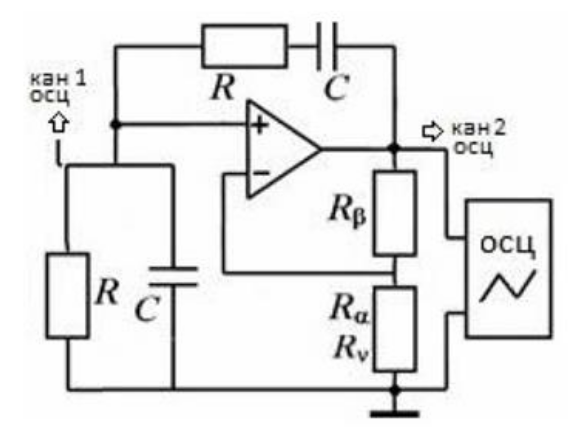
\includegraphics[width=0.5\textwidth]{27-4.png}
	\caption{Схема автогенератора}
\end{figure}

Характеристики устройств:
\[ R = 10 \, \text{кОм} \]
\[ C = 15 \, \text{нФ} \]
\[ R_\alpha = 188 \, \text{Ом} \]
\[ R_\beta = 393 \, \text{Ом} \]

Коэффициент усиления: 
\[ k = 1 + \dfrac{R_\beta}{R_\alpha} = 3.09 \]
Условие самовозбуждения \( k > 3 \) выполняется.

После включения питания мы сняли осциллограммы напряжений на выходе ОУ и на неинвертирующем входе ОУ.

Частота генерации: \( f_G = 924.37 \, \text{Гц} \)
Напряжения на входе и выходе: \( U_e = 2 \, \text{В}; \quad U_a = 6.6 \, \text{В} \)

Амплитуда колебаний на выходе ОУ равна 8 В.
Амплитуда колебаний на неинвертирующем входе ОУ равна 3.2 В.

\subsubsection*{Исследование автогенератора синусоидальных колебаний}

В предыдущей схеме заменили резистор \( R_\alpha \) терморезистором \( R_v \) (миниатюрной лампочкой накаливания). Проверим с помощью графика \( R_v(U) \) (рис. 5) выполнение условия самовозбуждения генератора при установленном в цепи резисторе \( R_\beta \).

\begin{figure}[htpb]
	\centering
	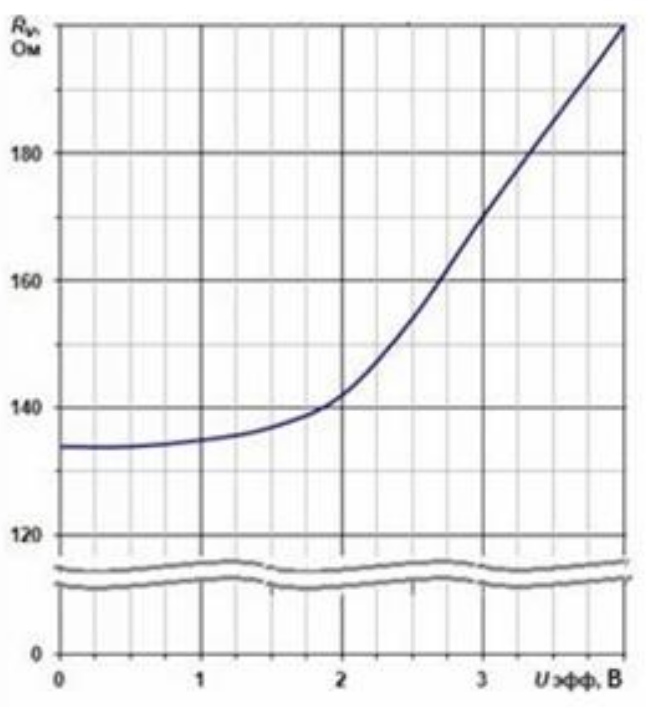
\includegraphics[width=0.3\textwidth]{27-5.png}
	\caption{Граифик зависимоти термосопротивления от напряжения}
\end{figure}

Были получены следующие осциллограммы напряжений на входе и выходе ОУ (рис. 6):

\begin{figure}[htpb]
	\centering
	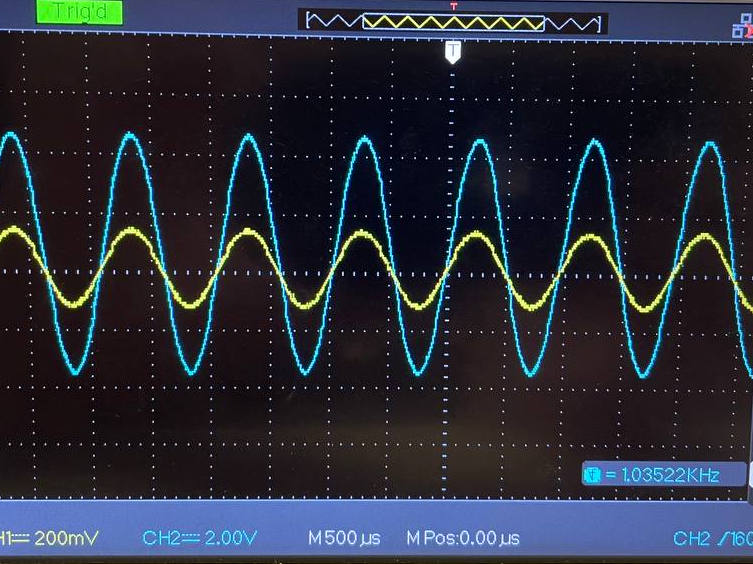
\includegraphics[width=0.5\textwidth]{27-5.jpg}
	\caption{Осцилограммы напряжений}
\end{figure}

Частота генерации: \( f_G = 924.31 \, \text{Гц} \)
Напряжения на входе и выходе: \( U_p = 2 \, \text{В}; \quad U_a = 6.8 \, \text{В} \)

Амплитуда колебаний на выходе ОУ равна 3.2 В.
Амплитуда колебаний на неинвертирующем входе ОУ равна 1 В.

Считаем, что инерция (скорость) нагрева существенно меньше скорости изменения токов и напряжений в цепи. Тогда для среднего коэффициента усиления действительна формула:

\[
K_c(U_p) = 1 + \dfrac{R_\beta}{R_v(U_p)} = 1 + \dfrac{393 \, \text{Ом}}{140 \, \text{Ом}} = 3.8
\]

Следовательно, условие самовозбуждения \( K_c(U_p) > 3 \) выполняется.

\subsubsection*{Снятие амплитудной характеристики}

В автогенераторе с терморезистором разорвали цепь обратной связи и подключили к входу неинвертирующего усилителя лабораторный генератор синусоидальных колебаний (рис. 7).

\begin{figure}
	\centering
	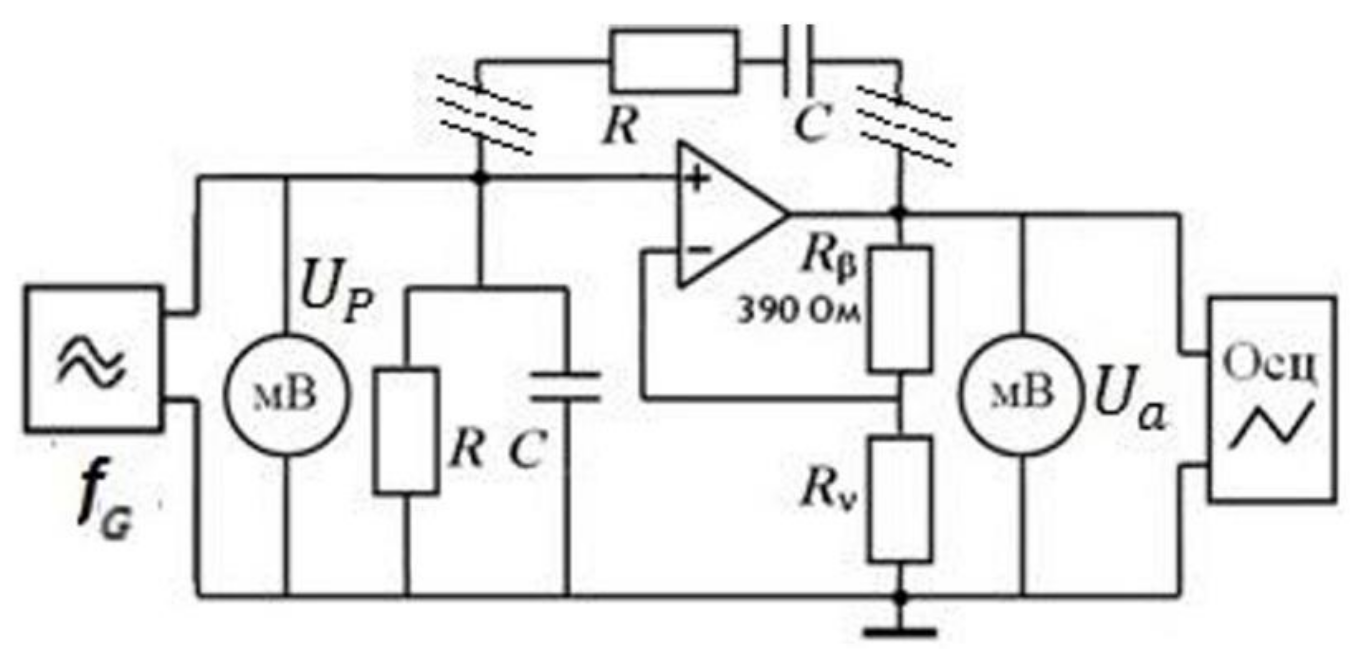
\includegraphics[width=0.5\textwidth]{27-7.png}
	\caption{Схема снятия амплитудной характеристики}
\end{figure}

Характеристики устройств:
\[ R = 10 \, \text{кОм} \]
\[ C = 15 \, \text{нФ} \]
\[ R_\beta = 393 \, \text{Ом} \]

Частоту колебаний установили равной частоте генерации \( f_G = 924.31 \, \text{Гц} \), измеренной в предыдущем опыте. После включили питание, и изменяя уровень напряжения генератора, сняли амплитудную характеристику \( U_a(U_p) \) (таблица №1):

\begin{table}[h]
	\centering
	\begin{tabular}{|c|c|c|c|}
		\hline
		№ & \( U_p, \, \text{В} \) & \( U_a, \, \text{В} \) & \( K_c(U_p) \) \\ \hline
		1 & 0.5 & 1.65 & 3.3 \\ \hline
		2 & 1.0 & 3.3 & 3.3 \\ \hline
		3 & 1.5 & 4.5 & 3.0 \\ \hline
		4 & 1.8 & 5 & 2.8 \\ \hline
		5 & 2.2 & 5.8 & 2.6 \\ \hline
		6 & 2.8 & 6.6 & 2.4 \\ \hline
	\end{tabular}
	\caption{Амплитудная характеристика \( U_a(U_p) \)}
\end{table}

Построим график зависимости среднего коэффициента усиления от действующего значения входного напряжения (рис. 8).

\begin{figure}[htpb]
	\centering
	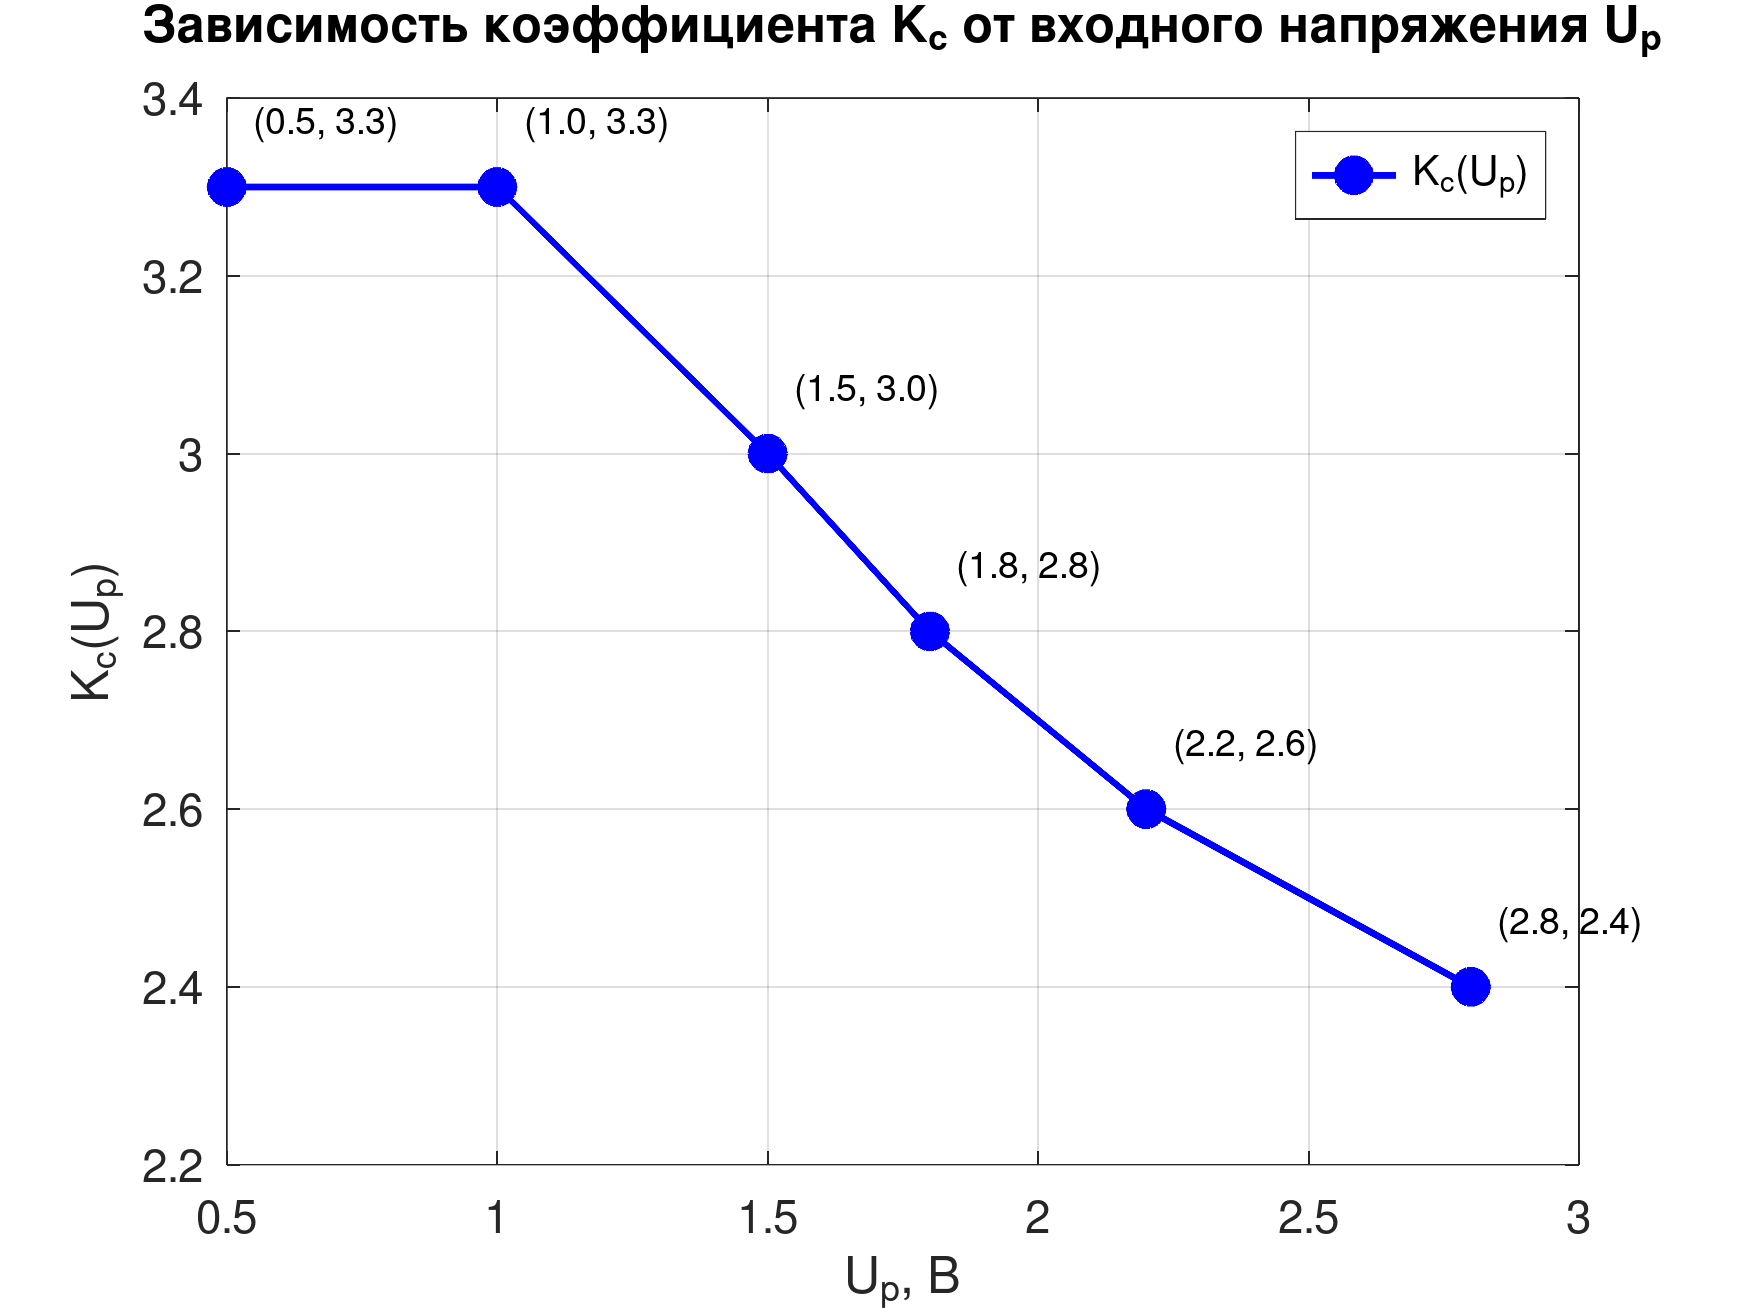
\includegraphics[width=0.6\textwidth]{27-8.png}
	\caption{График зависимости среднего коэффициента усиления от действующего значения
		входного напряжения}
\end{figure}

Действующие значения стационарных колебаний, полученные графическим методом решения уравнения баланса амплитуд (\( K_c(U_p) = 3 \)): 
\[ U_{pG} = 1.5 \, \text{В}; \quad U_{aG} = 4.5 \, \text{В} \]

Модуль погрешности амплитуды входного напряжения: 
\[ \dfrac{|U_a - U_{aG}|}{U_a} \times 100\% = \dfrac{|6.6 - 4.5|}{6.6} \times 100\% = 40.6\% \]
Данное значение превышает погрешность для резисторов и конденсаторов в 10\% в 4 раза.

Модуль погрешности амплитуды выходного напряжения: 
\[ \dfrac{|U_p - U_{pG}|}{U_p} \times 100\% = \dfrac{|2 - 1.5|}{2} \times 100\% = 50.0\% \]
Данное значение превышает погрешность для резисторов и конденсаторов в 10\% в 5 раз.

\subsubsection*{Исследование переходного процесса при самовозбуждении генератора}

На неинвертирующем усилителе с теми же резисторами \( R_\beta \) и \( R_v \) (см. рис. 3) построили генератор низкочастотных гармонических колебаний, выбрав резисторы и конденсаторы подходящих номиналов:

Характеристики устройств:
\[ R = 435 \, \text{кОм} \]
\[ C = 150 \, \text{нФ} \]
\[ R_\beta = 393 \, \text{Ом} \]

Квазирезонансная частота: 
\[ f_0 = \dfrac{1}{2\pi RC} = 2.44 \, \text{мГц} \]

Получена следующая осциллограмма выхода из состояния равновесия и развития автоколебаний при замыкании обратной связи и нулевых начальных условиях (нулевых напряжениях на конденсаторах) (рис. 9).

\begin{figure}[htpb]
	\centering
	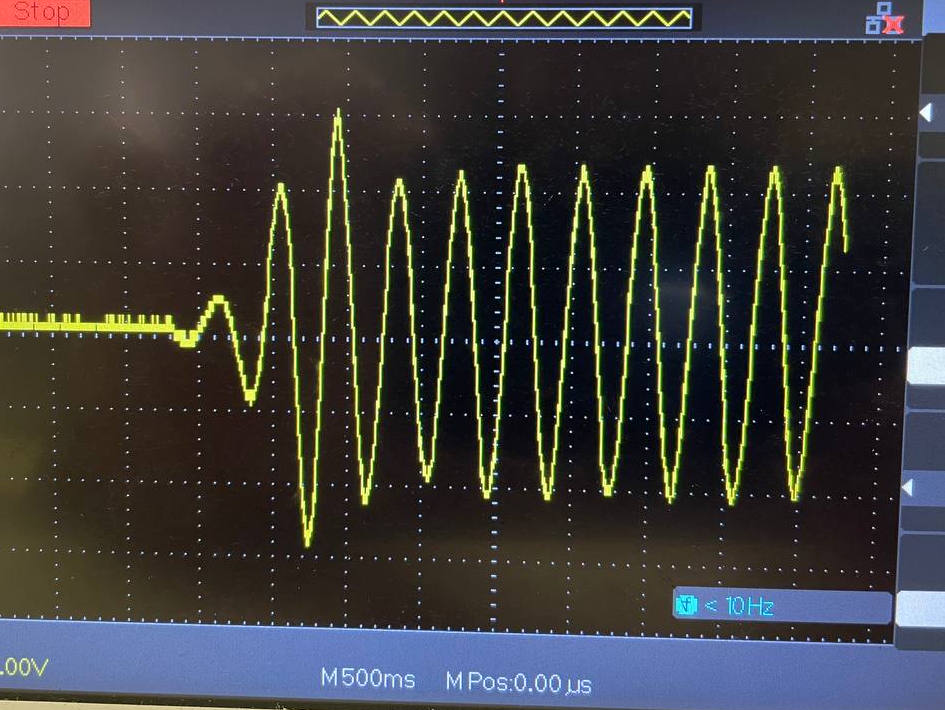
\includegraphics[width=0.6\textwidth]{27-9.jpg}
	\caption{Осциллограмма выхода из состояния равновесия и развития автоколебаний при
		замыкании обратной связи c $R_{\upsilon}$}
\end{figure}

Установившиеся синусоидальные автоколебания имеют амплитуду \( U_{aG} = 4.4 \, \text{В} \).

Заменили в исходной схеме резистор \( R_v \) на \( R_\alpha = 188 \, \text{Ом} \). Коэффициент усиления: 
\[ k = 1 + \dfrac{R_\beta}{R_\alpha} = 3.09 \]
Условие самовозбуждения \( k > 3 \) выполняется «на грани». Получили следующую осциллограмму (рис. 10).

\begin{figure}
	\centering
	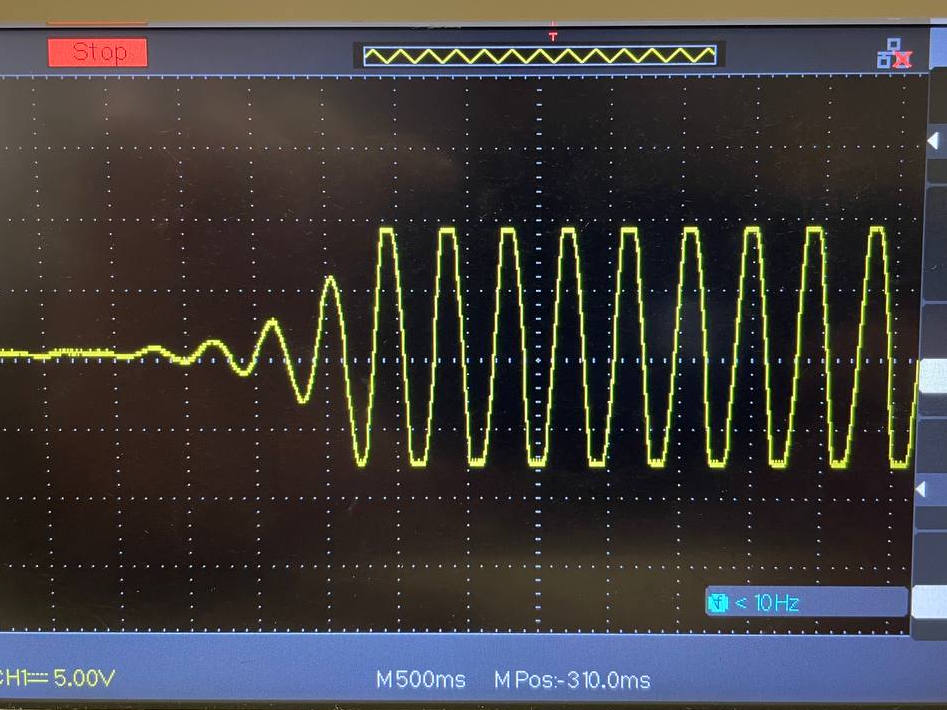
\includegraphics[width=0.6\textwidth]{27-10.jpg}
	\caption{Осциллограмма выхода из состояния равновесия и развития автоколебаний при
		замыкании обратной связи c $R_{\alpha}$}
\end{figure}

Установившиеся синусоидальные автоколебания имеют амплитуду \( U_{aG} = 9 \, \text{В} \).

Сравним и объясним особенности переходных процессов и установившихся режимов в RC-генераторах с обычными резисторами и с инерционной нелинейностью.

В случае использования резистора \( R_v \), т.е. когда \( k < 3 \), начальное возмущение убывает с ростом \( t \). В этом случае состояние покоя устойчиво. Это связано с положительным показателем экспоненты в уравнении гармонических колебаний, полученного из уравнения закона Кирхгофа.

В случае использования резистора \( R_\alpha \), т.е. когда \( k > 3 \), начальное возмущение растёт с ростом \( t \). Амплитуда нарастает по экспоненте до тех пор, пока \( u_p \) остаётся в пределах линейного участка передаточной характеристики НУ. Это связано с отрицательным показателем экспоненты в уравнении гармонических колебаний, полученного из уравнения закона Кирхгофа.

\subsubsection*{Вывод}

\subsubsection*{Пассивный RC-фильтр.} 
Теоретическая квазирезонансная частота \( f_0 = 1061.57 \, \text{Гц} \) отличается от экспериментальной \( f_{0\ эксп} = 935.84 \, \text{Гц} \) на 11.85\%. Данное значение превышает погрешность для резисторов и конденсаторов в 10\% на 1.85\%. Экспериментально полученный коэффициент передачи \( K_{\text{эксп}} = 0.3 \) отличается от теоретического \( K = 0.33 \) на 9.09\%. Данное значение не превышает погрешность для резисторов и конденсаторов в 10\%.

\subsubsection*{Избирательный усилитель.} 
Экспериментально полученный коэффициент передачи \( K_{\text{эксп}} = 25.5 \) отличается от теоретического \( K = 51.62 \) на 50.6\%. Данное значение превышает погрешность для резисторов и конденсаторов в 10\% в 5 раз. Экспериментально полученная добротность \( Q_{e\ эксп} = 7.39 \) отличается от теоретической \( Q_e = 12.5 \) на 40.9\%. Данное значение превышает погрешность для резисторов и конденсаторов в 10\% в 4 раза.

\subsubsection*{Автогенератор.} 
Для используемых в данной работе резисторов и конденсаторов значение коэффициента усиления, при котором выполнилось условие самовозбуждения, \( k = 3.09 \). Частота сгенерированных колебаний \( f_G = 924.37 \, \text{Гц} \). После замены в схеме (рис.~4) резистора \( R_\alpha \) на \( R_v \) мы наблюдаем стабилизацию амплитуды при той же частоте колебаний и значениях входного и выходного напряжения. При увеличении \( U_p \) сопротивление \( R_v \) растёт (рис.~5), снижая коэффициент усиления, что и обеспечило устойчивые колебания. В случае резистора \( R_\alpha \) амплитуда просто нарастала до насыщения.

\subsubsection*{Амплитудная характеристика.} 
Амплитудная характеристика (табл.~1 и рис.~8) подтверждает роль терморезистора как нелинейного элемента, обеспечивающего стабилизацию амплитуды автоколебаний. Снижение \( K_c \) при увеличении \( U_p \) предотвращает перегрев системы и выход ОУ в режим насыщения.

\subsubsection*{Переходные процессы.} 
При использовании терморезистора (рис.~9) переходный процесс быстро стабилизировался благодаря инерционному изменению сопротивления. С резистором \( R_\alpha \) (рис.~10) наблюдался экспоненциальный рост амплитуды.

В ходе работы подтвердилась необходимость использования нелинейных элементов для стабилизации автоколебаний.

\end{document}